8. \begin{figure}[ht!]
\center{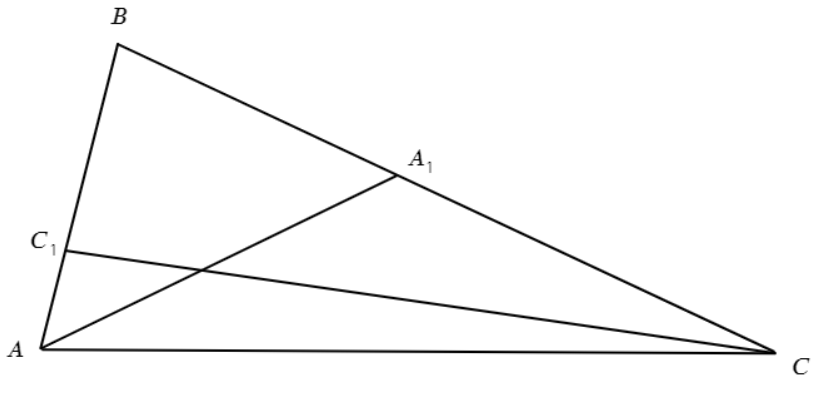
\includegraphics[scale=0.35]{g8.png}}
\end{figure}\\
Запишем четыре неравенства треугольника: $AB+BA_1>AA_1,\ AC+CA_1>AA_1,\ BC+BC_1>CC_1,\ AC+AC_1>CC_1.$ После сложения этих неравенств получим
$AB+AC+BC+AC+BA_1+CA_1+BC_1+AC_1>2AA_1+2CC_1,\ 2P>2AA_1+2CC_1,\ P>AA_1+CC_1,$ ч.т.д.\\
